\documentclass[12pt, a4paper, fleqn, titlepage]{article}
\usepackage[utf8]{inputenc}
\usepackage{hyperref}
\usepackage{graphicx}
\usepackage{algorithm}
\usepackage{algorithmic}
\usepackage{graphicx}
\graphicspath{ ./ }
\usepackage[margin=1in]{geometry}

\title{\textbf{CS 434: Parallel and Distributed Computing Lab 3}}
\author{Kweku Yamoah: 71712022}
\date{\today}

\begin{document}

\maketitle



\newpage
\section{Matrix Multiplication using MPI}
In this algorithm, I design a very simplistic approach of row-block partitioning and column-block partitioning onto P processors. Two matrices A and B are assumed to be square matrices to make computation easy utilising P number of processors. A is partitioned into $\sqrt{P}$ rows and matrix B is partitioned into $\sqrt{P}$ columns.\\
\subsection{Pseudocode overview}

All matrices are allocated memory. Matrices A and B are initlaised with integers, depending on the matrix size specified. The size represents the number of rows and columns, denoting a square matrix. So each matrix contains \emph{N x N} elemnts. \\

The next hurdle to overcome was the creation of rowtypes and cloumntypes. I used MPI Derived types achieve the create of these elements. The first step was to create a rowtype datatype. I did this by create an MPI subarray type with the displacements along $\sqrt{P}$ chunks. Hence each chunk has a dimension of $N x \sqrt{P}$\\

After, I scatter this row type to all processors so each processor will have it's local matrix to compute. The matrix I used for the scattering was A. The MPI method used was MPI\_Scatterv.\\

Similarlly, I created my cloumntype in a smilar fashion as my rowtype. I created my array to move along the columns of matrix B with a displacement of 1. This ensures that the cloumntype has the elements that reflect the corresponding rowtype elements. Then I scatter this datatype from matrix B to all processors.\\

With my elements scattered well to the correct processors, I go on to compute A x B using the matrix multiplication algorithm. But first, I had to reorient my cloumntype to ensure the computations are right. cloumntype are scattered in the form \emph{$\sqrt{P} * N$} but I need it in the form \emph{$N * \sqrt{P} $}. Hence the need for reorientation. \\

After all computations have be done on all processors, I gather the results into one matrix(C). Then I calculate the duration for all computations to take place.

\subsection{Limitations of Implementation}
The first limitation is I assume that \emph{N} the size of matrices is a number which is evenly divided by $\sqrt{P}$. Example; if N=8, then we need P=4 thereby $\sqrt{P}$ =2.Again,  if N=16, then we need P=8 thereby $\sqrt{P}$ =2(approximately). \\

I do this to in order to be able to distribute equal chunks of matrice elements to all processors for computations.Hence my advise to anyone running this program is that they should ensure that \textbf{P$= \frac{N}{2}$} at most. If this is not adhered to the code breaks.\\

Second limitation is that one cannot exceed the number of processors on the submachine they are running on. If you have a 32-core machine the highest P=32. Similarlly for 6
-core machines the highest P=64.



\subsection{Comparative Table}
    The table below shows the performance of the two versions as implemented in the C programming language.
    \begin{center}  
        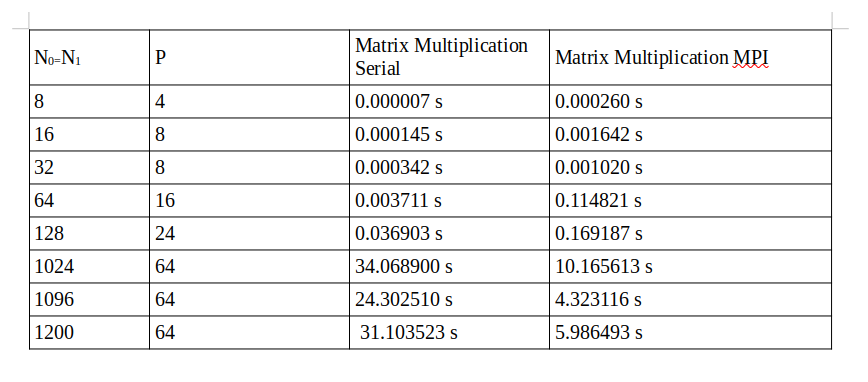
\includegraphics[width= 18cm,height = 10cm, keepaspectratio,scale=0.5]{lab3-table}
    \end{center}

    After generating the comparative table, I observed that for small sizes of N the serial Implementation of the matrix multiplication algorithm executed faster. However, as N grew exponentially, the parallel implementation in MPI executed faster than the serial implementation. This goes to show the importance of parallel computing and message passing communications in Computing.
\end{document}
